\documentclass[svgnames]{beamer}
\mode<presentation>
\usefonttheme{serif}
\usecolortheme{dove}
\useinnertheme{rounded}
\setbeamercolor{item projected}{fg=black}
\setbeamertemplate{navigation symbols}{}

\usepackage[english]{babel}
\usepackage[latin1]{inputenc}
\usepackage{times}
\usepackage{amsmath}
\usepackage{amsfonts}
\usepackage{amssymb}
\usepackage{amsthm}
\usepackage{graphicx}
\usepackage{multicol}
\usepackage{framed}
\usepackage{ulem}
\usepackage{ifthen}
\usepackage{tikz}
\usepackage{gastex}
\usepackage{ulem}
\usepackage{booktabs}

\newcommand{\set}[1]{\{ #1 \}}
\newcommand{\seq}[1]{\langle #1 \rangle}
\renewcommand{\P}{\mathcal{P}}
\newcommand{\FM}{\mathrm{FM}}
\newcommand{\SAT}{\mathrm{SAT}}
\newcommand{\crochet}[1]{\llbracket #1 \rrbracket}
\newcommand{\crochetc}[1]{\crochet{#1}^\textrm{c}}
\newcommand{\tree}{\mathrm{Tree}}

\newcommand{\At}{\mathbb{A}}
\newcommand{\Orb}{\mathcal{O}}
\newcommand{\A}{\mathcal{A}}
\newcommand{\Pred}{\mathcal{P}}
\newcommand{\N}{\mathbb{N}}
\newcommand{\Z}{\mathbb{Z}}
\newcommand{\Q}{\mathbb{Q}}
\newcommand{\D}{\mathbb{D}}
\newcommand{\M}{\mathcal{M}}
\newcommand{\FO}{\mathrm{FO}}
\newcommand{\NP}{\mathrm{NP}}
\newcommand{\co}{\mathrm{co}}
\newcommand{\PTIME}{\mathrm{PTIME}}
\newcommand{\EXPTIME}{\mathrm{EXPTIME}}
\newcommand{\MSO}{\mathrm{MSO}}
\newcommand{\Atoms}{\mathrm{Atoms}}
\newcommand{\Sym}{\mathrm{Sym}}
\newcommand{\sheet}{\mathrm{Sc}}
\newcommand{\col}{\mathrm{Color}}
\newcommand{\mem}{\mathrm{mem}}
\newcommand{\dom}{\mathrm{dom}}
\newcommand{\orb}{\mathrm{orb}}
\newcommand{\arity}{\mathrm{ar}}

\renewcommand{\ULthickness}{1.2pt}

%%%%%%%%%%%%%%%%%%%%%%%%%%%%%%%%%%%%%%%%%%%%%%%%%%%%%%%%%%%%%%%%%%%%%%%%%%%%%%%
%%%%%%%%%%%%%%%%%%%% A non-original creation by Nathana�l Fijalkow and myself %

\setbeamertemplate{frametitle}{%
  \vskip-2pt%
  \begin{beamercolorbox}[rightskip=2cm,leftskip=1em,dp=1ex,wd=12.8cm]{frametitle}%
    \vskip2pt%
    \usebeamercolor{frametitle}%
    \begin{tikzpicture}[scale=1]%
      \useasboundingbox (0,0) rectangle (0,0); %(-1,-1) rectangle (1,1);%
      \ifthenelse{\insertframenumber<\inserttotalframenumber}%
      { % uncomplete tart

        \pgfmathsetmacro{\aimangle}{90-(\insertframenumber*360/\inserttotalframenumber)}
        \fill [fill=frametitle.fg,thin, color=gray!50,draw=black] (11.8,.2) -- (11.8,.6) arc (90:\aimangle:0.4) -- cycle;%

      }{ % the full tart
        \fill[fill=frametitle.fg,thin, color=gray!50,draw=black] (11.8,0.2) circle (.4);%
      }%
      \fill[fill=frametitle.fg,thin, color=white,draw=black] (11.8,0.2) circle (.3);%
      \node at (11.8, .2) [black,circle]{\normalsize\insertframenumber};

    \end{tikzpicture}
    \insertframetitle%
    \vskip2pt%
  \end{beamercolorbox}%
}
%%%%%%%%%%%%%%%%%%%%%%%%%%%%%%%%%%%%%%%%%%%%%%%%%%%%%%%%%%%%%%%%%%%%%%%%%%%%%%%


\setbeamertemplate{blocks}[rounded]%
%[shadow=true]
\setbeamercolor{block title}{bg=normal text.bg!90!black}
\setbeamercolor{block body}{bg=normal text.bg!95!black}

\newtheorem{obs}{Observation}

\begin{document}

\addtocounter{framenumber}{-1}

\title{Boundedness problems in games: a roadmap}
\subtitle{GT Jeux'2012}
\author{Nathana\"el Fijalkow\\
(based on a joint work with Martin Zimmermann)}
\institute{Institute of Informatics, Warsaw University -- Poland 
\and LIAFA, Universit\'e Paris 7 Denis Diderot -- France}
\date{September 21st, 2012}

\begin{frame}
\maketitle
\end{frame}

\begin{frame}{Games with counter}
\begin{center}
Two-player turn-based games over \textbf{finite} graphs
\begin{picture}(60,65)(0,-4)
	\gasset{Nw=8,Nh=8}
	
  	\rpnode[polyangle=45](1)(30,15)(4,5){}
  	\node(2)(20,30){}
  	\node(3)(40,30){}
  	\rpnode[Nmarks=i,iangle=180,polyangle=45](4)(0,30)(4,5){}
  	\rpnode[polyangle=45](5)(10,50)(4,5){}
  	\node(6)(10,10){}
  	\rpnode[polyangle=45](7)(30,50)(4,5){}

  	\drawedge(1,2){}
  	\drawedge[curvedepth=3](1,3){}
	\drawloop[loopangle=90](2){}
  	\drawedge(2,3){}
  	\drawedge(2,6){}
  	\drawedge[curvedepth=5](3,1){}
  	\drawedge(4,2){}
  	\drawedge[curvedepth=5](4,5){}
  	\drawedge[curvedepth=5](5,4){}
	\drawloop[loopangle=-90](6){}
  	\drawedge(7,5){}

\begin{huge}
\only<2,3>{\put(60,20){$c_2 \doteq 0$}}
\only<2,3>{\put(60,40){$c_1 \doteq 0$}}
\end{huge}

\only<3>{
  	\drawedge(1,2){$i,\varepsilon$}
  	\drawedge[curvedepth=3](1,3){$\varepsilon,r$}
	\drawloop[loopangle=90](2){$i,i$}
  	\drawedge(2,3){$\varepsilon,\varepsilon$}
  	\drawedge[ELside=r](2,6){$r,r$}
  	\drawedge[curvedepth=5](3,1){$r,i$}
  	\drawedge(4,2){$\varepsilon,r$}
  	\drawedge[curvedepth=5](4,5){$\varepsilon,i$}
  	\drawedge[ELside=r,curvedepth=5](5,4){$i,i$}
	\drawloop[loopangle=-90](6){$\varepsilon,r$}
  	\drawedge[ELside=r](7,5){$i,\varepsilon$}
	}
	
\end{picture}
\end{center}
\pause
Winning condition: ``there exists B, such that $\ldots$''
\end{frame}

\begin{frame}{Actions on the counters}
\begin{framed}
\textbf{increment:}
$i$ or ``$c \longleftarrow c+1$''
\end{framed}

\begin{framed}
\textbf{no action:}
$\varepsilon$
\end{framed}

\begin{framed}
\textbf{reset:}
$r$ or ``$c \longleftarrow 0$''
\end{framed}

\begin{framed}
\textbf{decrement:}
``$c \longleftarrow c-1$''
\end{framed}

\begin{framed}
\textbf{refill:}
``$c \longleftarrow c+\omega$''
\end{framed}
\end{frame}

\begin{frame}{Roadmap}
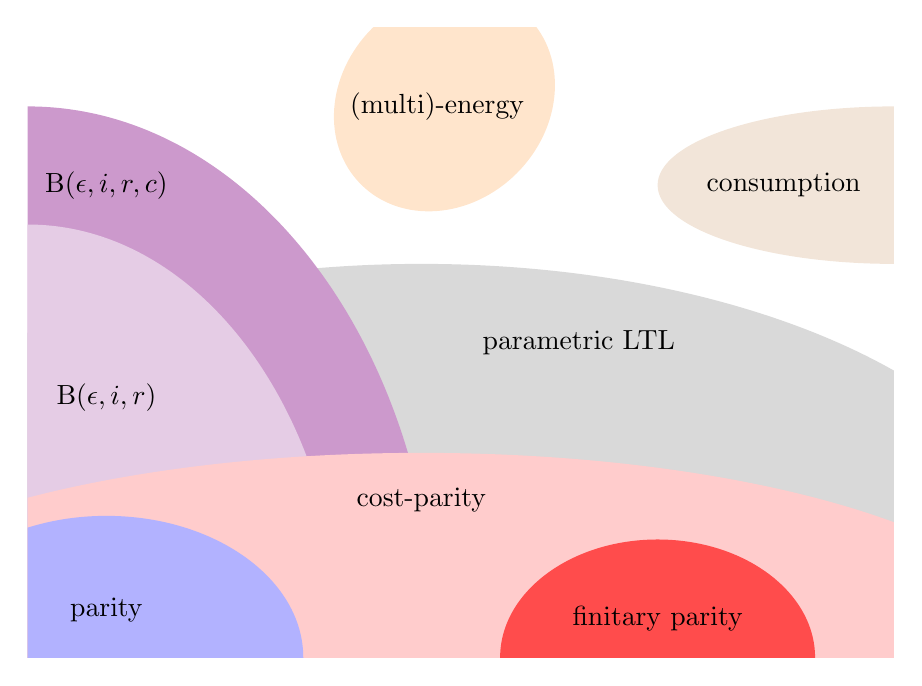
\begin{tikzpicture}
\clip (-6,0) rectangle (5,8);

\fill[white!85!black] (-1,1) ellipse (8cm and 4cm) ;
\draw (1,4) node {parametric LTL} ;

\fill[white!60!violet] (-6,0) ellipse (5.2cm and 7cm) ;
\draw (-5,6) node {B($\epsilon,i,r,c$)} ;

\fill[white!80!violet] (-6,0) ellipse (4cm and 5.5cm) ;
\draw (-5,3.3) node {B($\epsilon,i,r$)} ;

\fill[white!80!red] (-1,0) ellipse (8cm and 2.6cm) ;
\draw (-1,2) node {cost-parity} ;

\fill[white!70!blue] (-5,0) ellipse (2.5cm and 1.8cm) ;
\draw (-5,.6) node {parity} ;

\fill[white!30!red] (2,0) ellipse (2cm and 1.5cm) ;
\draw (2,.5) node {finitary parity} ;

\fill[white!80!brown] (5,6) ellipse (3cm and 1cm) ;
\draw (3.6,6) node {consumption} ;

\fill[white!80!orange,rotate=45] (4.5,5.5) ellipse (1.5cm and 1.3cm) ;
\draw (-.8,7) node {(multi)-energy} ;

\end{tikzpicture}
\end{frame}

\begin{frame}{The robust: $B$-conditions (Boja\'nczyk, Colcombet)}
Actions: $\varepsilon,i,r$.
\vskip2em

$B$-conditions are conjunctions of:
\begin{itemize}
	\item ``counter $c$ is bounded''\\
	\item B\"uchi($F$):\qquad ``$F$ appears infinitely often''\\
	\item CoB\"uchi($G$):\qquad ``$G$ appears finitely often''
\end{itemize}

\pause
\begin{obs}
\begin{center}
Eve wins ``counter $c$ is bounded''\\
if and only if\\
she wins ``B\"uchi($i$) $\Rightarrow$ B\"uchi($r$)''.
\end{center}
\end{obs}
\pause
\begin{corollary}
One can decide who wins a $B$-game and Eve needs finite memory.
\end{corollary}
\end{frame}

\begin{frame}{Roadmap}
\addtocounter{framenumber}{-1}
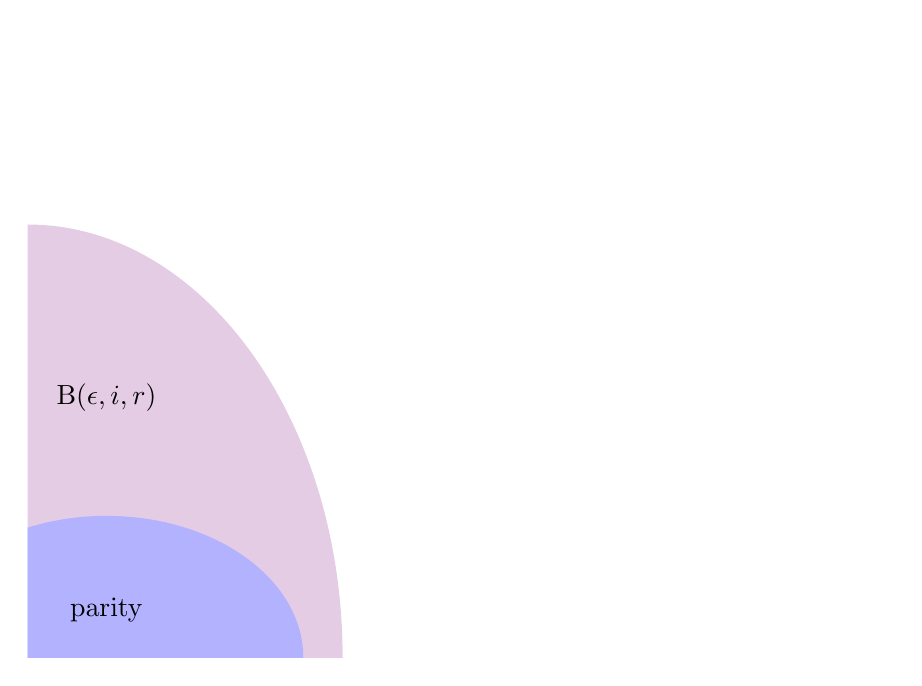
\begin{tikzpicture}
\clip (-6,0) rectangle (5,8);

\fill[white!80!violet] (-6,0) ellipse (4cm and 5.5cm) ;
\draw (-5,3.3) node {B($\epsilon,i,r$)} ;

\fill[white!70!blue] (-5,0) ellipse (2.5cm and 1.8cm) ;
\draw (-5,.6) node {parity} ;
\end{tikzpicture}
\end{frame}

\begin{frame}{The surprising: finitary parity (Alur,Henzinger)}

\begin{multicols}{2}
\begin{picture}(30,60)(0,0)
	\gasset{Nw=8,Nh=8}

  	\rpnode[polyangle=45](1)(30,15)(4,5){{\color{red}{$1$}}}
  	\node(2)(20,30){{\color{blue}{$2$}}}
  	\node(3)(40,30){{\color{red}{$3$}}}
  	\rpnode[Nmarks=i,iangle=180,polyangle=45](4)(0,30)(4,5){{\color{red}{$3$}}}
  	\rpnode[polyangle=45](5)(10,50)(4,5){{\color{blue}{$2$}}}
  	\node(6)(10,10){{\color{blue}{$4$}}}
  	\rpnode[polyangle=45](7)(30,50)(4,5){{\color{blue}{$0$}}}

  	\drawedge(1,2){}
  	\drawedge[curvedepth=3](1,3){}
	\drawloop[loopangle=90](2){}
  	\drawedge(2,3){}
  	\drawedge(2,6){}
  	\drawedge[curvedepth=5](3,1){}
  	\drawedge(4,2){}
  	\drawedge[curvedepth=5](4,5){}
  	\drawedge[curvedepth=5](5,4){}
	\drawloop[loopangle=-90](6){}
  	\drawedge(7,5){}
\end{picture}

\only<2>{
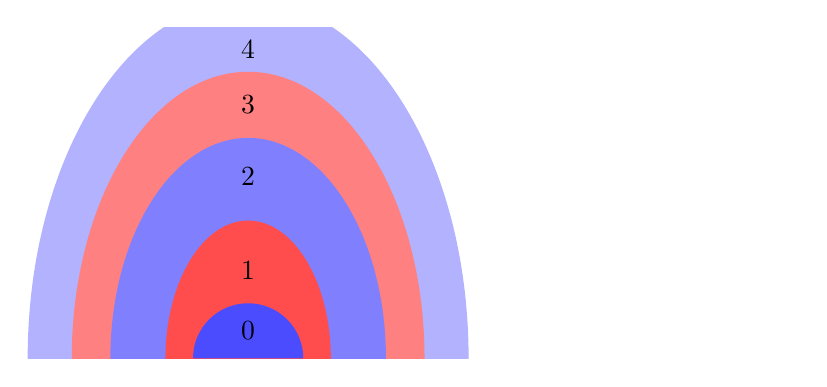
\begin{tikzpicture}[scale=.7]
\clip (-4,0) rectangle (10,6);

\fill[white!70!blue] (0,0) ellipse (4cm and 6.5cm) ;
\draw (0,5.6) node {$4$} ;

\fill[white!50!red] (0,0) ellipse (3.2cm and 5.2cm) ;
\draw (0,4.6) node {$3$} ;

\fill[white!50!blue] (0,0) ellipse (2.5cm and 4cm) ;
\draw (0,3.3) node {$2$} ;

\fill[white!30!red] (0,0) ellipse (1.5cm and 2.5cm) ;
\draw (0,1.6) node {$1$} ;

\fill[white!30!blue] (-1,0) arc (180:0:1) ;
\node at (0,.5) {$0$};
\end{tikzpicture}
\qquad {\color{red}{Requests}} \quad \qquad 
{\color{blue}{Responses}}
\vspace*{5cm}
}

\only<3>{

\begin{framed}
\textbf{Parity:}\\
Almost all requests are answered.
\end{framed}

\begin{framed}
\textbf{Finitary parity:}\\
There exists a bound $b$, s.t.\\
almost all requests are answered \textit{within $b$ steps}.
\end{framed}
\vspace*{10cm}
	}
\end{multicols}

\end{frame}

\begin{frame}{Parity games and finitary parity games are different}

\begin{multicols}{2}
\begin{framed}
\textbf{Parity:}\\
Almost all requests are answered.
\end{framed}
	
\begin{framed}
\textbf{Finitary parity:}\\
There exists a bound $b$, s.t.\\
almost all requests are answered \textit{within $b$ steps}.
\end{framed}
\vspace*{10em}
\end{multicols}

\only<1>{
\begin{center}
\begin{picture}(40,15)(0,0)
	\gasset{Nw=8,Nh=8}

  	\node(1)(0,5){{\color{red}{$1$}}}
  	\rpnode[polyangle=45](2)(20,10)(4,5){{\color{blue}{$2$}}}
  	\node(0)(40,5){{\color{blue}{$0$}}}

  	\drawedge(1,2){}
	\drawloop[loopangle=90](2){}
  	\drawedge(2,0){}
  	\drawedge[curvedepth=5](0,1){}
\end{picture}
\end{center}
Eve wins for the parity condition, 
\begin{flushright}
but loses for the finitary parity condition!
\end{flushright}
	}

\only<2>{
\begin{multicols}{2}
\begin{itemize}
	\item Both players have positional winning strategies.
	\item Deciding the winner is in $\NP \cap \co\NP$.
\end{itemize}
\vspace*{1em}

\begin{itemize}
	\item Eve has positional winning strategies.
	\item Adam needs infinite memory.
	\item Deciding the winner is in $\PTIME$.
\end{itemize}
\vspace*{3em}
\end{multicols}
	}

\end{frame}

\begin{frame}{Roadmap}
\addtocounter{framenumber}{-1}
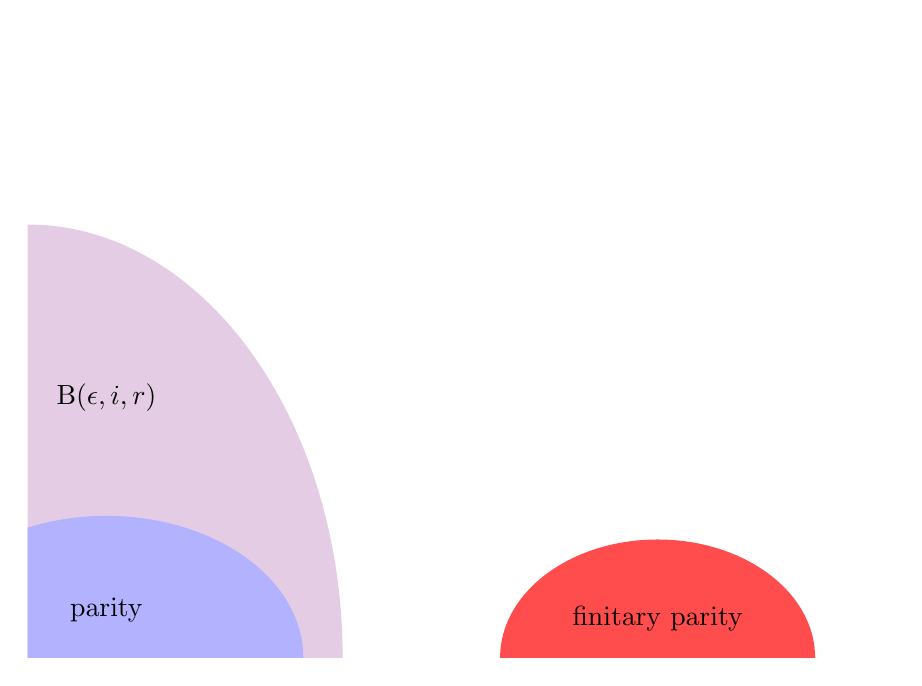
\begin{tikzpicture}
\clip (-6,0) rectangle (5,8);

\fill[white!80!violet] (-6,0) ellipse (4cm and 5.5cm) ;
\draw (-5,3.3) node {B($\epsilon,i,r$)} ;

\fill[white!70!blue] (-5,0) ellipse (2.5cm and 1.8cm) ;
\draw (-5,.6) node {parity} ;

\fill[white!30!red] (2,0) ellipse (2cm and 1.5cm) ;
\draw (2,.5) node {finitary parity} ;

\end{tikzpicture}
\end{frame}

\begin{frame}{Roadmap}
\addtocounter{framenumber}{-1}
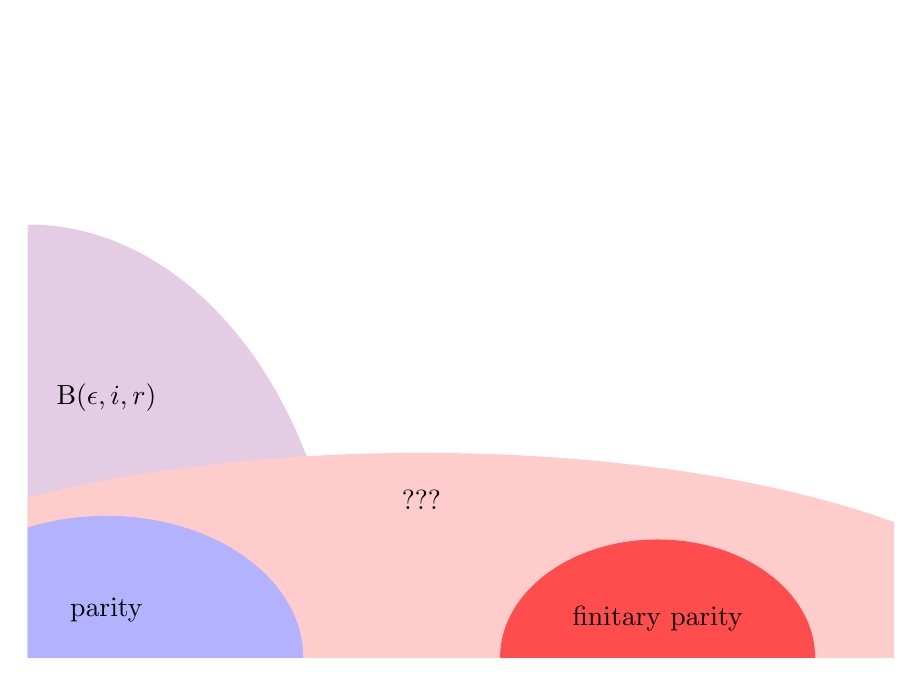
\begin{tikzpicture}
\clip (-6,0) rectangle (5,8);

\fill[white!80!violet] (-6,0) ellipse (4cm and 5.5cm) ;
\draw (-5,3.3) node {B($\epsilon,i,r$)} ;

\fill[white!80!red] (-1,0) ellipse (8cm and 2.6cm) ;
\draw (-1,2) node {???} ;
	
\fill[white!70!blue] (-5,0) ellipse (2.5cm and 1.8cm) ;
\draw (-5,.6) node {parity} ;

\fill[white!30!red] (2,0) ellipse (2cm and 1.5cm) ;
\draw (2,.5) node {finitary parity} ;

\end{tikzpicture}
\end{frame}

\begin{frame}{Cost-parity conditions}

\begin{center}
\begin{multicols}{2}
\begin{framed}
\textbf{Parity:}\\
Almost all requests are answered.
\end{framed}

\begin{framed}
\textbf{Finitary parity:}\\
There exists a bound $b$, s.t.\\
almost all requests are answered \textit{within $b$ steps}.
\end{framed}
\end{multicols}

\pause

\begin{framed}
\textbf{Cost-parity:}\\
There exists a bound $b$, s.t.\\
almost all requests are answered \textit{with cost at most $b$}.
\end{framed}
\end{center}

\end{frame}

\begin{frame}{Costs}

\begin{center}
\begin{picture}(80,45)(0,0)
	\gasset{Nw=6,Nh=6}

  	\node(1)(0,40){{\color{red}{$1$}}}
  	\rpnode[polyangle=45](2)(15,45)(4,5){{\color{blue}{$2$}}}
  	\node(0)(30,40){{\color{blue}{$0$}}}
	\put(5,27){Parity game}

  	\drawedge(1,2){$\varepsilon$}
	\drawloop[loopangle=90](2){$\varepsilon$}
  	\drawedge(2,0){$\varepsilon$}
  	\drawedge[curvedepth=5](0,1){$\varepsilon$}

  	\node(1b)(50,40){{\color{red}{$1$}}}
  	\rpnode[polyangle=45](2b)(65,45)(4,5){{\color{blue}{$2$}}}
  	\node(0b)(80,40){{\color{blue}{$0$}}}
	\put(50,27){Finitary parity game}

  	\drawedge(1b,2b){i}
	\drawloop[loopangle=90](2b){i}
  	\drawedge(2b,0b){i}
  	\drawedge[curvedepth=5](0b,1b){i}

  	\node(1bb)(25,0){{\color{red}{$1$}}}
  	\rpnode[polyangle=45](2bb)(40,5)(4,5){{\color{blue}{$2$}}}
  	\node(0bb)(55,0){{\color{blue}{$0$}}}

  	\drawedge(1bb,2bb){i}
	\drawloop[loopangle=90](2bb){$\varepsilon$}
  	\drawedge(2bb,0bb){i}
  	\drawedge[curvedepth=5](0bb,1bb){$\varepsilon$}
\end{picture}
\end{center}

\end{frame}

\begin{frame}{Roadmap}
\addtocounter{framenumber}{-1}
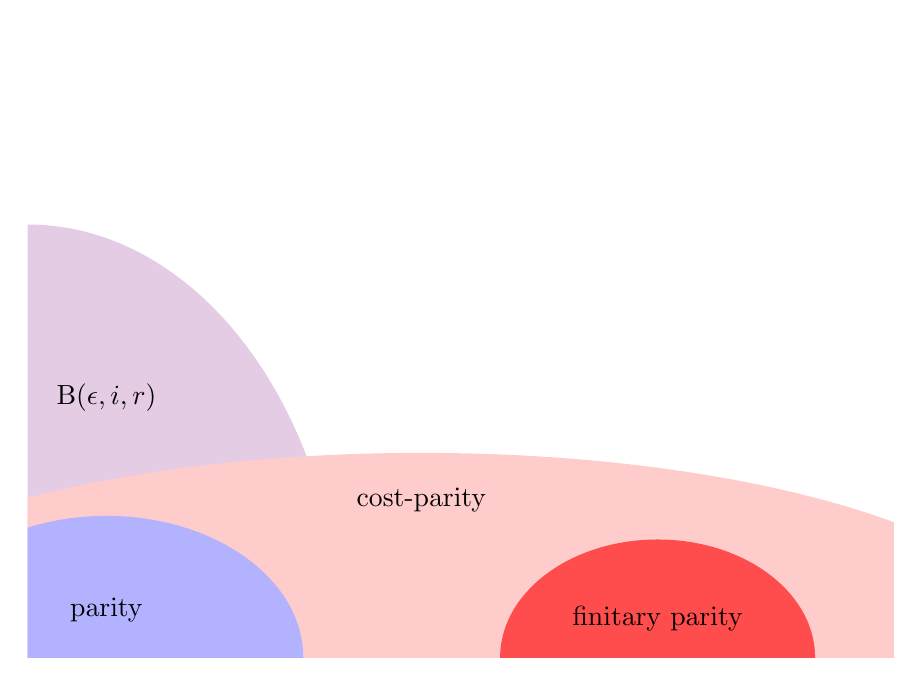
\begin{tikzpicture}
\clip (-6,0) rectangle (5,8);

\fill[white!80!violet] (-6,0) ellipse (4cm and 5.5cm) ;
\draw (-5,3.3) node {B($\epsilon,i,r$)} ;

\fill[white!80!red] (-1,0) ellipse (8cm and 2.6cm) ;
\draw (-1,2) node {cost-parity} ;
	
\fill[white!70!blue] (-5,0) ellipse (2.5cm and 1.8cm) ;
\draw (-5,.6) node {parity} ;

\fill[white!30!red] (2,0) ellipse (2cm and 1.5cm) ;
\draw (2,.5) node {finitary parity} ;

\end{tikzpicture}
\end{frame}

\begin{frame}{Deciding the winner in cost-parity games}
$n$: number of vertices\\
$m$: number of edges\\
$d$: number of colors
\vskip2em
\begin{theorem}[F.,\ Zimmermann 2012]
Given a parity games solver of complexity $T(n,m,d)$,\\
we construct a cost-parity games solver of complexity 
$$O(n \cdot T(n \cdot d,m \cdot d,d+2))\ .$$
\end{theorem}
\end{frame}

\begin{frame}{Positional determinacy for Eve}
Objective: \textbf{strategy optimization}\\
\begin{framed}
Assume $\sigma$ is a winning strategy.\\
How to construct a memoryless winning strategy $\sigma'$ from $\sigma$?
\end{framed}
\pause
Tool: \textbf{scoring functions}
\vskip2em
``\`a la M\"uller and Schupp'' past-oriented proof
\end{frame}

\begin{frame}{Roadmap}
\addtocounter{framenumber}{-1}
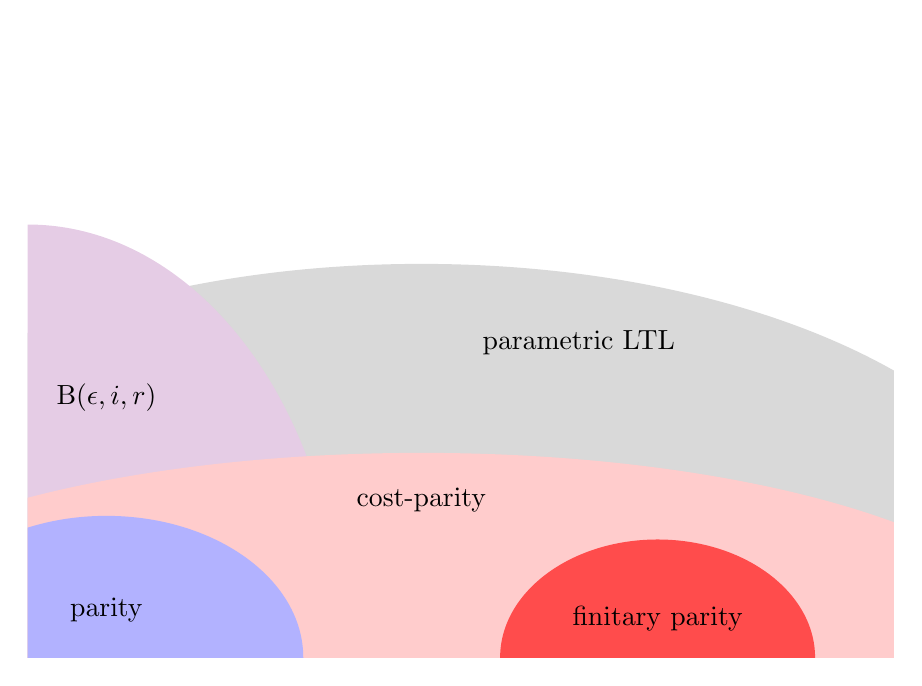
\begin{tikzpicture}
\clip (-6,0) rectangle (5,8);

\fill[white!85!black] (-1,1) ellipse (8cm and 4cm) ;
\draw (1,4) node {parametric LTL} ;

%\fill[white!60!violet] (-6,0) ellipse (5.2cm and 7cm) ;
%\draw (-5,6) node {B($\epsilon,i,r,c$)} ;

\fill[white!80!violet] (-6,0) ellipse (4cm and 5.5cm) ;
\draw (-5,3.3) node {B($\epsilon,i,r$)} ;

\fill[white!80!red] (-1,0) ellipse (8cm and 2.6cm) ;
\draw (-1,2) node {cost-parity} ;

\fill[white!70!blue] (-5,0) ellipse (2.5cm and 1.8cm) ;
\draw (-5,.6) node {parity} ;

\fill[white!30!red] (2,0) ellipse (2cm and 1.5cm) ;
\draw (2,.5) node {finitary parity} ;

%\fill[white!80!brown] (5,6) ellipse (3cm and 1cm) ;
%\draw (3.6,6) node {consumption} ;
%
%\fill[white!80!orange,rotate=45] (4.5,5.5) ellipse (1.5cm and 1.3cm) ;
%\draw (-.8,7) node {(multi)-energy} ;

\end{tikzpicture}
\end{frame}

\begin{frame}{Roadmap}
\addtocounter{framenumber}{-1}
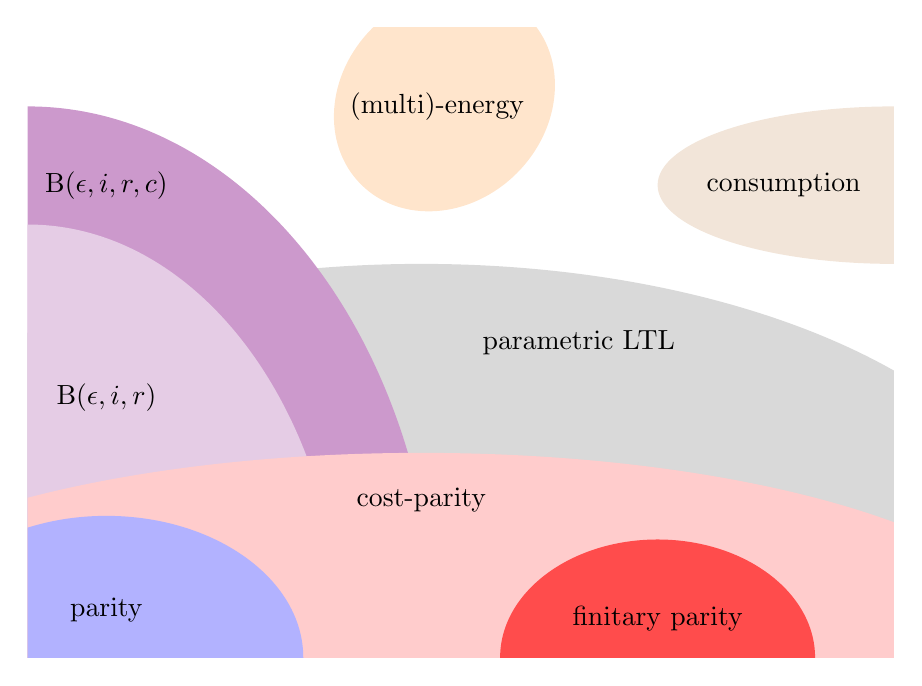
\begin{tikzpicture}
\clip (-6,0) rectangle (5,8);

\fill[white!85!black] (-1,1) ellipse (8cm and 4cm) ;
\draw (1,4) node {parametric LTL} ;

\fill[white!60!violet] (-6,0) ellipse (5.2cm and 7cm) ;
\draw (-5,6) node {B($\epsilon,i,r,c$)} ;

\fill[white!80!violet] (-6,0) ellipse (4cm and 5.5cm) ;
\draw (-5,3.3) node {B($\epsilon,i,r$)} ;

\fill[white!80!red] (-1,0) ellipse (8cm and 2.6cm) ;
\draw (-1,2) node {cost-parity} ;

\fill[white!70!blue] (-5,0) ellipse (2.5cm and 1.8cm) ;
\draw (-5,.6) node {parity} ;

\fill[white!30!red] (2,0) ellipse (2cm and 1.5cm) ;
\draw (2,.5) node {finitary parity} ;

\fill[white!80!brown] (5,6) ellipse (3cm and 1cm) ;
\draw (3.6,6) node {consumption} ;

\fill[white!80!orange,rotate=45] (4.5,5.5) ellipse (1.5cm and 1.3cm) ;
\draw (-.8,7) node {(multi)-energy} ;

\end{tikzpicture}
\end{frame}

\begin{frame}{Multi-energy}

\begin{framed}
\textbf{increment:}
$i$ or ``$c \longleftarrow c+1$''
\end{framed}

\begin{framed}
\textbf{no action:}
$\varepsilon$
\end{framed}

\begin{framed}
\textbf{decrement:}
``$c \longleftarrow c-1$''
\end{framed}

\vskip2em
\begin{small}
(Tom\'a\v{s} Br\'azdil, Jakub Chaloupka, Krishnendu Chatterjee, Laurent Doyen, 
Uli Fahrenberg, Petr Jan\v{c}ar, Line Juhl, Anton\'in Ku\v{c}era, 
Kim G. Larsen, Jean-Fran\c cois Raskin, Mickael Randour, Ji\v{r}i Srba,$\ldots$)
\end{small}

\end{frame}

\begin{frame}{Consumption}
\begin{framed}
\sout{\textbf{increment:}
$i$ or ``$c \longleftarrow c+1$''}
\end{framed}

\begin{framed}
\textbf{no action:}
$\varepsilon$
\end{framed}

\begin{framed}
\textbf{decrement:}
``$c \longleftarrow c-1$''
\end{framed}

\begin{framed}
\textbf{refill:}
``$c \longleftarrow c+\omega$''
\end{framed}

\begin{small}
(Tom\'a\v{s} Br\'azdil, Krishnendu Chatterjee, Anton\'in Ku\v{c}era, Petr Novotn�, CAV'2012)
\end{small}
\end{frame}

\begin{frame}{$B$-conditions with checks}

\textbf{check:}
``counter $c$ is bounded on \textbf{checked} values''

\begin{framed}
\textbf{increment:}
$i$ or ``$c \longleftarrow c+1$''
\end{framed}

\begin{framed}
\textbf{no action:}
$\varepsilon$
\end{framed}

\begin{framed}
\textbf{reset:}
``$c \longleftarrow 0$''
\end{framed}

\begin{framed}
\textbf{max:}
``$c \longleftarrow \max(c',c'')$''
\end{framed}

\end{frame}

\begin{frame}{Roadmap}
\addtocounter{framenumber}{-1}
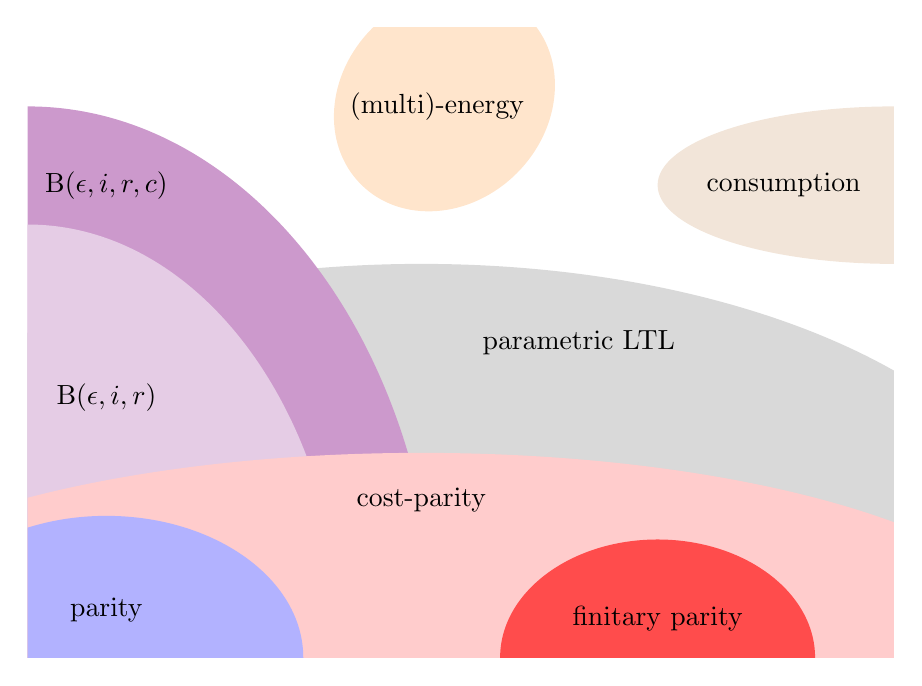
\begin{tikzpicture}
\clip (-6,0) rectangle (5,8);

\fill[white!85!black] (-1,1) ellipse (8cm and 4cm) ;
\draw (1,4) node {parametric LTL} ;

\fill[white!60!violet] (-6,0) ellipse (5.2cm and 7cm) ;
\draw (-5,6) node {B($\epsilon,i,r,c$)} ;

\fill[white!80!violet] (-6,0) ellipse (4cm and 5.5cm) ;
\draw (-5,3.3) node {B($\epsilon,i,r$)} ;

\fill[white!80!red] (-1,0) ellipse (8cm and 2.6cm) ;
\draw (-1,2) node {cost-parity} ;

\fill[white!70!blue] (-5,0) ellipse (2.5cm and 1.8cm) ;
\draw (-5,.6) node {parity} ;

\fill[white!30!red] (2,0) ellipse (2cm and 1.5cm) ;
\draw (2,.5) node {finitary parity} ;

\fill[white!80!brown] (5,6) ellipse (3cm and 1cm) ;
\draw (3.6,6) node {consumption} ;

\fill[white!80!orange,rotate=45] (4.5,5.5) ellipse (1.5cm and 1.3cm) ;
\draw (-.8,7) node {(multi)-energy} ;

\end{tikzpicture}
\end{frame}

\end{document}

\begin{frame}{A general framework}
\addtocounter{framenumber}{-1}
Consider a winning strategy $\sigma : V^* \rightarrow V$.
\vskip1em
Define a scoring function $\sheet : V^* \rightarrow (S,\le)$ satisfying:
\pause
\begin{enumerate}
	\item $(S,\le)$ is a total order and $\sheet$ is a congruence:\\
	if $\sheet(w) \le \sheet(w')$, 
	then $\sheet(w \cdot v) \le \sheet(w' \cdot v)$.
\vskip1em
\pause
	\item If there exists a bound~$b$ such that the scores of all prefixes of a play~$\rho$ are bounded
	by $b$, then $\rho$ is winning.
\vskip1em
\pause
	\item Assume a play $\rho$ is consistent with $\sigma$, 
	then the scores of all prefixes of $\rho$ are (uniformly) bounded.
\end{enumerate}
\pause
\vskip1em
Construct a memoryless strategy $\sigma'$: 
\begin{center}
``play according to $\sigma$ assuming the worst play prefix''.
\end{center}
\end{frame}

\begin{frame}{Results (FSTTCS'2012)}
\addtocounter{framenumber}{-1}
$$\begin{array}{llll}
\toprule
\textrm{winning condition} & \textrm{complexity} & \textrm{Player } 0 & \textrm{Player } 1 \\
\midrule
\textrm{parity} & {\color{red}{\NP \cap \co\NP}} & {\color{red}{\textrm{memoryless}}} & \textrm{memoryless} \\
\textrm{finitary parity} & \PTIME & {\color{red}{\textrm{memoryless}}} & {\color{red}{\textrm{infinite}}} \\
\textrm{cost-parity} & \NP \cap \co\NP & \textrm{memoryless} & \textrm{infinite} \\
\midrule
\textrm{Streett} & \co\NP\textrm{-complete} & {\color{red}{\textrm{finite}}} & \textrm{memoryless} \\
\textrm{finitary Streett} & {\color{red}{\EXPTIME\textrm{-complete}}} & {\color{red}{\textrm{finite}}} & {\color{red}{\textrm{infinite}}} \\
\textrm{cost-Streett} & \EXPTIME\textrm{-complete} & \textrm{finite} & \textrm{infinite} \\
\bottomrule
\end{array}$$
\end{frame}

